% Created 2020-06-16 Tue 19:48
% Intended LaTeX compiler: pdflatex
% Template: Diogo Ferrari
\documentclass[a4paper]{article}
% === Packages =================================
\usepackage{./sty/basic-article}
\usepackage{./sty/math-commands}
\usepackage{./sty/math-commands-thm}
% === Document =================================
\author{Diogo Ferarri}
\date{\today}
\title{}
\hypersetup{
 pdfauthor={Diogo Ferarri},
 pdftitle={},
 pdfkeywords={},
 pdfsubject={},
 pdfcreator={Emacs 26.3 (Org mode 9.0.9)}, 
 pdflang={English}}
\begin{document}

\tableofcontents



\section{Guidelines}
\label{sec:orgd293b17}
You can find guidelines in the folder \texttt{./guidelines/} to help you to write final papers, final research projects, and presentations. Below you find some suggestions of tools that are commonly used in academia.

\section{Latex and Beamer}
\label{sec:org19dbf74}

From \(\LaTeX\) \href{https://www.latex-project.org/}{webiste}:

\begin{quote}


\LaTeX{} is a high-quality typesetting system; it includes features designed for technical and scientific writing. \LaTeX{} is the de facto standard for the communication and publication of scientific documents.
\end{quote}

If you are new to \LaTeX, read \href{https://www.latex-tutorial.com/}{this} document to get started. There are many tutorials on that website to help you to learn \LaTeX. Another good source is \href{https://scholar.harvard.edu/mkomisarchik/tutorials-0}{this} tutorial by Mayya Komisarchik. You can also find some examples and templates in the folder \texttt{./latex-and-beamer/}.


\href{https://en.wikipedia.org/wiki/Beamer\_(LaTeX)}{Beamer} is a latex document class that you can use to create professional-looking presentations. \href{https://www.overleaf.com/learn/latex/Beamer\_Presentations:\_A\_Tutorial\_for\_Beginners\_(Part\_1)\%E2\%80\%94Getting\_Started}{Here} is a good tutorial to learn how to use it. You can find some examples and templates in the folder \texttt{./latex-and-beamer/}.

It is a good idea to invest on learning \href{https://en.wikipedia.org/wiki/Comparison\_of\_reference\_management\_software}{reference management} to organize your bibliography. All those softwares for reference management either store or can export references in \href{https://en.wikipedia.org/wiki/BibTeX}{.bib} format. That format is nicely integrated with \LaTeX. Organizing references in .bib files make it much easier to cite previous work and include references.

\section{Statistical Programming: R and Python}
\label{sec:org4e9a6ff}
Here are some useful resources to learn R:

\begin{description}
\item[{\href{https://style.tidyverse.org/}{R style guide} (Tideverse)}] (free) some tips about how to structure your code to make it more readable and reproducible.
\item[{\href{https://r4ds.had.co.nz/}{R for Data Science}}] (free) introductory-level book written by \href{http://hadley.nz/}{Hadley Wickham}, Chief Scientist at RStudio, and an Adjunct Professor of Statistics at the University of Auckland, Stanford University, and Rice University. The website of the book contains examples and includes instructions to work with pipe and tydeverse. The latter is a popular package ecosystem for data analysis and dataviz.
\end{description}


Here are some useful resources to learn Python:

\begin{description}
\item[{\href{https://www.python.org/dev/peps/pep-0008/}{Python Style Guide}}] (free) some tips about how to structure your code to make it more readable and reproducible.
\item[{Downey (2015)}] (free) good introductory-level book with the most important concepts and code examples in Python.
\end{description}
\section{Project Management}
\label{sec:orgeafa053}
\subsection{Project Folder Structure}
\label{sec:org73b6a13}
It is a good idea to use a consistent folder structure to organize your research and software projects. That will make it easier to (1) navigate the folder structure to find files, (2) re-run and replicate the analysis later, (3) distribute your code and files for replication. I keep all past projects in a folder called \texttt{projects\_archive} and all current projects in a folder named \texttt{projects}. Each project gets its own subfolder. For instance, if I am currently working on a projects \texttt{social-cognition} and another one called \texttt{hdpglm}, I will have these two subfolders in the \texttt{projects} folder:

\begin{center}
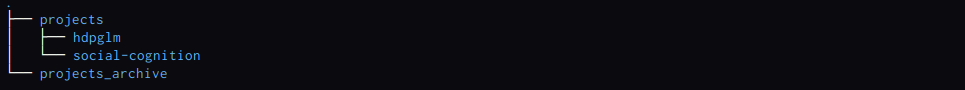
\includegraphics[width=1\textwidth]{./project-management/project-structure-master.png}
\end{center}


Each project, by its turn, contains the same set of subfolders, although the file names may differ in each project. For instance, the folders and files inside the directory for the \texttt{social-cognition} project, or equivalently inside the directory \texttt{hdpglm}, will have the following basic structure:

\begin{center}
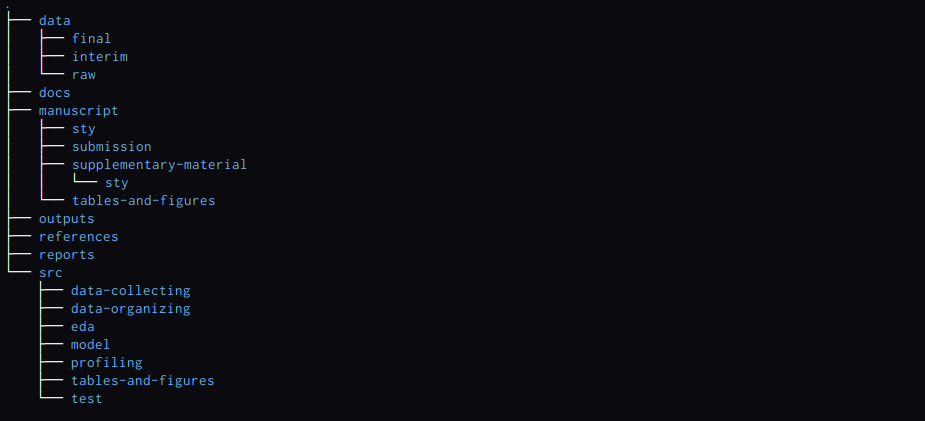
\includegraphics[width=1\textwidth]{./project-management/project-structure.png}
\end{center}

The content of each folder is the following:

\begin{center}
\begin{tabular}{llp{9cm}}
\hline
\hline
Folder & Subfolder & Content\\
\hline
\hline
data & ./final & contains the final version of the data set used for the analysis\\
 & ./interim & contains intermediate data sets created to explore the data, merge ,etc. The raw data after some recoding and manipulation by scripts in the folder \texttt{.src/} go here\\
 & ./raw & contains the raw data sets as collected from external sources\\
\hline
docs &  & contains documents related to the project, such as grant proposal, codebooks of the data sets, etc.\\
\hline
manuscript & ./ & file with papers written for the project\\
 & ./sty & latex sty file I used to compile the papers\\
 & ./submission & contains versions of the papers submitted to journals. I create subfolders with the name of the journals to store the version submitted to that journal\\
 & ./supplementary-material & all supplementary material, including figures and latex files\\
 & ./tables-and-figures & all .tex tables and figures I used in the papers\\
\hline
outputs & ./ & files with the outputs of analyses. Usually, .Rout files and .log, but also files with simulated data sets\\
\hline
references & ./ & I keep all my .pdf files with papers and books in a single folder shared by all projects. In this folder, I keep files that are related to the project and that I use as reference, such as handouts, reports written by other scholars on the topic, etc.\\
\hline
reports & ./ & Reports I create for the project, such as exploratory data analysis\\
\hline
src &  & scripts will go in subfolders of this folder\\
 & ./data-collecting & scripts I used to collect the raw data\\
 & ./data-organizing & scripts I used for data wrangling and to create interim and final data sets from raw data\\
 & ./eda & scripts I used for exploratory data analysis, prior to final analysis\\
 & ./model & scripts that produce the final results and analysis.\\
 & ./tables-and-figures & I use this folder in case I create temporary tables and figures\\
 & ./test & A folder for running tests in the code\\
\hline
\hline
\end{tabular}
\end{center}


\subsection{Git and Github}
\label{sec:org13116e9}
Version control softwares are very useful for production. Bryan (2018) contains some points about using version control. One of the most common version control software is \href{https://git-scm.com/}{Git}. It can be used to keep track of changes you make to files and scripts. \href{https://github.com/}{GitHub} is a could platform that uses git. You can find a very nice introductory material \href{https://www.elegantthemes.com/blog/resources/git-and-github-a-beginners-guide-for-complete-newbies}{here}.


\section{Integrated Development Environment (IDE)}
\label{sec:orgd794cc1}

You can write scripts as plain text for \LaTeX, Python, R, and Stata in any text editor. You will be better off, however, if you used an Integrated Development Environment (IDE). IDE are softwares written to facilite code writing. The choce is personal, but here are some good options:

Here are the main classical options:

\begin{itemize}
\item \href{https://www.gnu.org/software/emacs/}{Emacs}: this is my personal choice. I use emacs for everything, including writing code in Latex, Python, R, academic papers, books, create presentations, organize and manage citation and references (with bibtex), communicate with HPC servers, organize my schedule using org-mode (a "package" to use with emacs), and so on. It is highly configurable, but dull at its out-of-the-box raw state, without configuration. It takes quite some time to learn and unleash all its potential, but it is worth the time invested.
\item \href{https://www.vim.org/}{Vim}: main emacs competitor. Good, but not as resourceful.
\end{itemize}


Some good out-of-the-box and readyand-easy-to-use IDEs are:
\begin{itemize}
\item \href{https://rstudio.com/}{RStudio}: very easy to use and the barrier of entry is low. Good to write scripts in R.
\item \href{https://www.sublimetext.com/}{Sublime}: good for many programming languages, including R and Python. Also easy to use.
\item \href{https://atom.io/}{Atom}: like Sublime
\item \href{https://jupyter.org/}{Juputer Notebook}: it runs on web browsers, and can be used with many programming languages. There is anice tutorial \href{https://www.dataquest.io/blog/jupyter-notebook-tutorial/}{here}.
\item \href{http://texstudio.sourceforge.net/}{TexStudio}: good for writing code in Latex.
\end{itemize}


\section{References}
\label{sec:org7388575}
\begin{itemize}
\item Bryan, J. (2018). Excuse Me, Do You Have A Moment To Talk About Version Control?, \textit{The American Statistician}, 72(1), 20–27. (\url{https://peerj.com/preprints/3159v2/})
\item Downey, A. (2015). Think Python, : O'reilly Media, Inc.
\end{itemize}
\end{document}
